%Correct the file name.
%X: book number
%Y: part number
%ZZZ: page number in three digits. So page 3 would be 003.

\documentclass[11pt]{amsbook}

\usepackage{../HBSuerDemir}	% ------------------------
\usepackage{amsmath, wrapfig}

\begin{document}

\hPage{b2p1/129}
\par Then


\[
A.B=a_1b_1+a_2b_2+a_3b_3
\]

If the vectors are written as row and column vectors

\[
A=	 \begin{bmatrix}
       a_1 & a_2 & a_3           
     \end{bmatrix},   
B=	 \begin{bmatrix}
       b_1 \\
       b_2 \\
       b_3           
     \end{bmatrix}       
\]

then

\[
AB= \begin{bmatrix}
       a_1 & a_2 & a_3           
     \end{bmatrix}   
	 \begin{bmatrix}
       b_1 \\
       b_2 \\
       b_3           
     \end{bmatrix}
     =\begin{bmatrix}
     a_1b_1 & a_2b_2 & a_3b_3
     \end{bmatrix}
     =A.B
\]     

\par \underline{Example 1}. Given the vectors

\[
	A = (2, -3, 4), B = (5, 6, -1)
\]

find
\begin{wrapfigure}{r}{5.5cm}
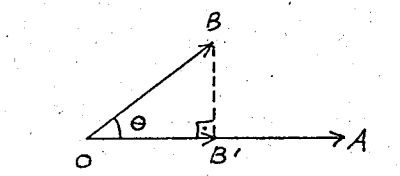
\includegraphics[width=0.45\textwidth]{images/b2p1-129-fig01}
\end{wrapfigure}
\paragraph{ a) scalar projection of B on A }
\paragraph{ b) vector projection of B on A }
\paragraph{ c) angle between A and B \\}

\paragraph{ \underline{Solution}. \\}
\paragraph{ a) $ A.B = |A| |B| \cos\vartheta $}

\[
	\Rightarrow  2.5 + (-3)6 + 4(-1) = \sqrt{4+9+16} \vec{|OB|} \cos\vartheta
\]
\[
	\Rightarrow -12=\sqrt{29}\vec{|OB|} \cos\vartheta
\]
\[
	\vec{|OB|} \cos\vartheta= \frac{-12}{\sqrt{29}}
\]

b) $\vec{OB'}=  \frac{-12}{\sqrt{29}} \frac{A}{|A|}$ ( A/$|A|$ is the unit vector in the direction and sense of A)
\[
=- \frac{12}{29} \frac{(2, -3, 4)}{\sqrt{29}} =( -\frac{24}{29}, \frac{36}{29}, -\frac{48}{29} )
\]




 
%\begin{figure}[h]
%	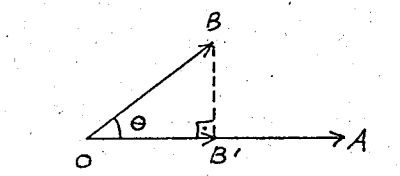
\includegraphics[width=0.45\textwidth]{images/b2p1-129-fig01}
%	\caption{Classification of complex numbers}
%	\label{fig:classificationOfComplexNumbersA}
%\end{figure}






% =======================================================
\end{document}  

%==== templates ====

%==== environments ====

%\begin{figure}[htb]
%	\centering
%	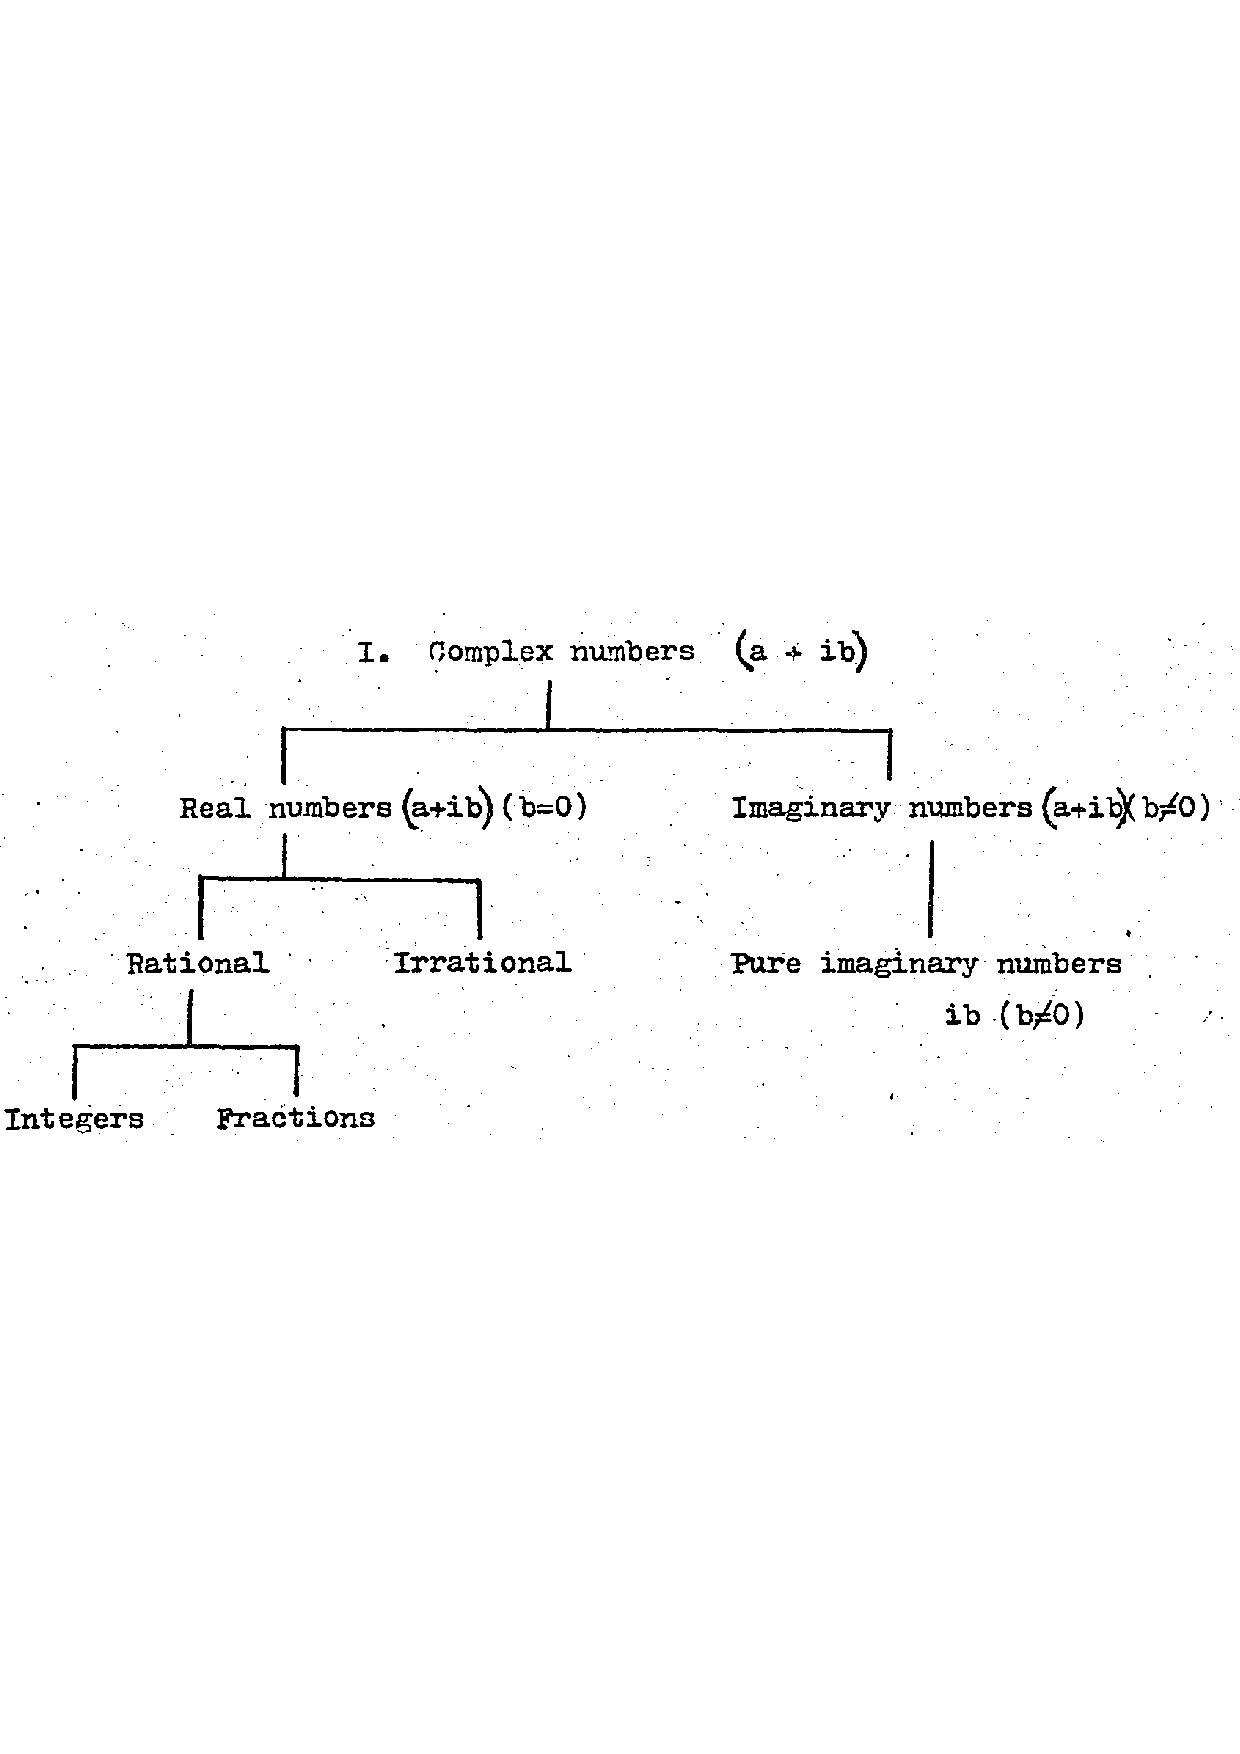
\includegraphics[width=0.9\textwidth]{images/SD-1-1p15A}
%	\caption{Classification of complex numbers}
%	\label{fig:classificationOfComplexNumbersA}
%\end{figure}

%\begin{center}
%\begin{tabular}{cc}
%\end{tabular}
%\end{center}

%\begin{exmp}
%\begin{hSolution}
%\end{hSolution}
%\end{exmp}

%\begin{hEnumerateAlpha}
%\end{hEnumerateAlpha}

%\begin{hEnumerateRoman}
%\end{hEnumerateRoman}

%$
%\begin{bmatrix}
%\end{bmatrix}
%$

%\frac{aaaa}{bbb}
%\frac{a_{n}}{b_{n}}
%\left( aaaa \right)
%\Longrightarrow

%\begin{multicols}{2}
%	bb
%\columnbreak
%	aa
%\end{multicols}
